\documentclass[10pt,letterpaper]{article}
\usepackage[letterpaper,top=1in,bottom=1in,left=1.05in,right=1.05in]{geometry}
\usepackage[T1]{fontenc}
\usepackage{amsmath}
\usepackage{txfonts}
\usepackage[expansion=false]{microtype}
\usepackage{parskip}
\usepackage{tikz}
\usetikzlibrary{arrows.meta,positioning,calc,fit}
\usepackage{booktabs,tabularx,array}
\usepackage{caption}
\usepackage{float}
\usepackage{listings}
\usepackage{url}
\usepackage[hidelinks]{hyperref}

\captionsetup{font=small,labelfont=bf,labelsep=period}
\setlength{\parskip}{0.55em}
\linespread{1.04}
\pagestyle{plain}
\emergencystretch=1.5em

\makeatletter
\renewcommand\section{\@startsection{section}{1}{\z@}{-1.3em}{0.45em}{\normalfont\large\bfseries}}
\renewcommand\subsection{\@startsection{subsection}{2}{\z@}{-0.9em}{0.25em}{\normalfont\normalsize\bfseries}}
\renewcommand\thesection{\arabic{section}.}
\renewcommand\thesubsection{\arabic{section}.\arabic{subsection}}
\renewcommand\@seccntformat[1]{\csname the#1\endcsname\ }
\makeatother

\lstset{basicstyle=\ttfamily\footnotesize,columns=fullflexible,keepspaces=true,
  frame=none,xleftmargin=1.5em,aboveskip=0.4em,belowskip=0.2em,showstringspaces=false}

\newcommand{\ak}{\mathsf{ak}}
\newcommand{\ask}{\mathsf{ask}}
\newcommand{\nk}{\mathsf{nk}}
\newcommand{\rivk}{\mathsf{rivk}}
\newcommand{\ivk}{\mathsf{ivk}}
\newcommand{\ovk}{\mathsf{ovk}}
\newcommand{\rk}{\mathsf{rk}}
\newcommand{\rsk}{\mathsf{rsk}}
\newcommand{\fvk}{\mathsf{FVK}}
\newcommand{\Gor}{\mathcal{G}}
\newcommand{\ytilde}{\tilde{y}}
\newcommand{\fn}[1]{\texttt{#1}}
\newcommand{\hx}[1]{\texttt{\small #1}}

\begin{document}

\begin{center}
{\Large\bfseries Cloakroom: A Peer-to-Peer Dark Pool for Shielded Zcash}\\[1.1em]
{\normalsize Chris Gachau}\\[0.25em]
{\small October 2026}
\end{center}

\vspace{0.4em}
\begin{quote}
\small
\textbf{Abstract.} A purely private version of exchange would allow shielded Zcash to be traded
for other assets without ever leaving the shielded pool. Today every route out of shielded ZEC
passes through a transparent address controlled by a custodian, a bridge, or an intent network,
which publishes amounts and timing and can hold funds. Atomic swaps remove the custodian, but the
hash-locked construction needs scripts that Zcash's shielded pools do not have, and it links both
legs of a trade with a shared hash. We propose a swap in which the ZEC never touches a transparent
address. The two parties split the spend authorizing key of a fresh Ironwood address into
additive shares; the counterparty's tokens are locked on an EVM chain in a contract with two exits,
each opened by revealing exactly one share. Whichever exit is taken publishes the share the other
party is missing, so the trade either settles on both sides or is refunded on both sides. On Zcash
the swap is two ordinary fully shielded transactions; on the EVM chain it reveals the price. A
request-for-quote protocol carried in encrypted memos turns the swap into a dark pool in which the
price is public and the participants are not. We implemented the protocol and ran it end to end:
against the production \fn{orchard} verifier, on a local Zebra node, in seven two-party
scenarios (five of them adversarial), and in two swaps between Zcash testnet and Base Sepolia, in which every Zcash
transaction was fully shielded.
\end{quote}

\section{Introduction}

Zcash~\cite{zerocash,spec} gives its users two kinds of money. Transparent value behaves like
Bitcoin~\cite{bitcoin}: every address, amount and transfer is public. Shielded value lives in a pool
of encrypted notes, and a fully shielded transaction shows an observer only that it happened and
what fee it paid. Most shielded ZEC now sits in the Ironwood pool, which the NU6.3 upgrade
introduced in July 2026~\cite{zip258}.

Shielded value stays private only while it stays shielded. Each crossing between the transparent
and shielded pools publishes the amount moved and when it moved, and matching crossings by amount
and timing has linked a large share of shielded activity to transparent
addresses~\cite{kappos,quesnelle,biryukov}; the same methods recently linked 17.65\% of withdrawals
from Railgun on Ethereum~\cite{railgun}. Exchange is where the crossings happen. Major exchanges
withdraw ZEC only to transparent addresses. NEAR Intents, the most used swap route, supports ZEC on
transparent addresses only~\cite{nearchains}, and Maya and THORChain hold ZEC in transparent
vaults. Every route also adds a custodian: in 2026 one user's \$589{,}000 USDT payout from a ZEC
swap was held by NEAR Intents in a compliance review for more than fifty days~\cite{freeze}, and on
October~1 NEAR Intents was exploited for about \$3.8 million and paused~\cite{nearexploit}.

Atomic swaps~\cite{nolan,herlihy} remove the custodian, but the usual construction locks both legs to
the same hash preimage behind a timelock. Zcash's shielded pools have no script system, so the lock
has to sit on transparent outputs, where it publishes the amount, and the shared hash then appears on
both chains and links the two legs~\cite{xcat}. Monero, which also lacks scripts, solved this
differently: the Monero leg is sent to an address whose spending key is split between the parties,
and the other leg is built so that taking it reveals the missing share~\cite{gugger,athanor}.

We apply that idea to the Orchard protocol, which the Ironwood pool uses, and build a market on top
of it. Our contributions are:
\begin{itemize}\setlength\itemsep{0.1em}
\item A swap between shielded ZEC and any EVM token whose Zcash leg is two ordinary fully shielded
transactions and never uses a transparent address (Sections~4 and~5).
\item An EVM escrow that checks a revealed scalar against a stored Pallas point directly, so no
cross-curve equality proof is needed (Section~4.3).
\item An analysis that names what each observer learns, including three pitfalls that are easy to
miss: the shared outgoing viewing key, the fact that a reverted transaction still publishes its
secret, and the light-wallet server learning which transactions are ours (Sections~5 to~7).
\item A request-for-quote protocol in 512-byte encrypted memos (Section~8).
\item An implementation, and evidence at four levels: the production verifier, a local Zebra node,
seven two-party scenarios, and two swaps on public test networks (Sections~9 and~10).
\end{itemize}

\section{Background}

\subsection{Orchard keys}
The Orchard protocol~\cite[\S4.2.3]{spec} works over the Pallas curve $E_p: y^2 = x^3 + 5$, whose
group has prime order $q$. A spending key yields a \emph{spend authorizing key}
$\ask \in \mathbb{F}_q^*$, a \emph{nullifier deriving key} $\nk \in \mathbb{F}_p$, and a
\emph{commitment randomness} $\rivk \in \mathbb{F}_q$. The \emph{spend validating key} is
$\ak = [\ask]\,\Gor$, where $\Gor$ is the RedPallas spend-authorization base point
$\mathsf{GroupHash}(\texttt{"z.cash:Orchard"}, \texttt{"G"})$. A full viewing key encodes $\ak$ by
its $x$-coordinate alone~\cite[\S5.6.4.4]{spec}, so key generation fixes the sign of its
$y$-coordinate: if $\ytilde(\ak) = 1$, $\ask$ is negated. The triple $(\ak, \nk, \rivk)$ is the full
viewing key. From it come the incoming viewing key
$\ivk = \mathsf{Commit}^{\ivk}_{\rivk}(\mathsf{Extract}(\ak), \nk)$, which must not be $0$ or $\bot$;
an outgoing viewing key $\ovk$, derived with $\rivk$ as a PRF key; and an unbounded family of mutually
unlinkable \emph{diversified addresses} $(d, \mathsf{pk}_d = [\ivk]\,g_d)$.

\subsection{Spending}
A shielded transaction is a set of \emph{actions}, each pairing one spend with one
output~\cite{spec}. To spend a note, the spender picks a fresh randomizer $\alpha$, publishes the
randomized key $\rk = \ak + [\alpha]\Gor$, and signs the transaction's ZIP~244
sighash~\cite{zip244} with RedPallas under $\rsk = \ask + \alpha$. A Halo~2 proof~\cite{halo} shows,
without saying which note is spent, that $\rk$ randomizes the $\ak$ behind that note's address, that
the note is in the commitment tree, and that the published nullifier is correct. Because $\alpha$ is
uniform, $\rk$ is a uniform point that reveals nothing about $\ak$. An action publishes only a value
commitment, a nullifier, $\rk$, a note commitment, an ephemeral key, two ciphertexts and a signature,
and the bundle adds a proof and a binding signature.

\subsection{Partially created transactions}
A partially created Zcash transaction (PCZT)~\cite{zip374} lets different machines construct,
prove and sign a transaction. A Signer receives each action's $\alpha$ and the sighash; the
\fn{orchard} crate accepts an externally produced signature only if it verifies under $\rk$.
Threshold signing for Zcash, FROST~\cite{frost,zip312}, uses this interface to spend from a key that
no single machine holds.

\subsection{Ironwood and NU7}
In May 2026 a soundness flaw was found in the Orchard circuit. NU6.2 deployed a fixed circuit, and
NU6.3 (``Ironwood'', July~28, 2026) introduced a new pool that uses the fixed circuit, and sealed the
old Orchard pool so value can only leave it~\cite{zip258}. Ironwood reuses the Orchard key structure
and address format, and one incoming viewing key scans both pools~\cite{zip326}. ZIP~2005 adds an
optional key derivation, $\mathsf{use\_qsk}$, that makes notes recoverable in a quantum
emergency~\cite{zip2005}. NU7 has been active on testnet since October~4, 2026 and is scheduled for
mainnet; it shortens the block interval to 25~seconds and keeps the transaction format~\cite{zip259}.

\section{Related Work}

\textbf{Hash-locked swaps.} Nolan's 2013 construction~\cite{nolan}, formalized by
Herlihy~\cite{herlihy}, and the 2017 Zcash--Bitcoin XCAT~\cite{xcat} need a script that checks a hash
preimage and a timelock. In Zcash this exists only for transparent outputs.

\textbf{Monero swaps.} Gugger~\cite{gugger} showed that a chain without scripts can be swapped
against Bitcoin if its leg is locked to a key split between the parties and the Bitcoin leg uses
adaptor signatures to reveal a share, with two timelocks $t_0$ and $t_1$. COMIT ran the protocol in
production from 2021~\cite{comit}; the project continues as eigenwallet. AthanorLabs replaced the
Bitcoin leg with an Ethereum contract that checks a revealed secp256k1 scalar~\cite{athanor}.
Because Monero keys live on Ed25519, that design also needs a proof that one scalar underlies points
on both curves~\cite{mrl10}. Our escrow checks the Pallas point directly. Its windows also differ:
AthanorLabs allows a claim when ready before $t_0$ or between $t_0$ and $t_1$; we allow a claim
whenever the swap is ready, up to $t_1$, which shortens the happy path and opens no race, because
refunds are closed from Ready until $t_1$.

\textbf{Other designs.} Universal atomic swaps~\cite{uas} need only signature verification on each
chain and use adaptor signatures with time-lock puzzles; since Orchard spend authorization is a
Schnorr-type signature they could in principle apply to shielded ZEC, but we know of no RedPallas
implementation. Zswap~\cite{zswappets} is a different scheme with a similar name: multi-asset
swaps inside a single shielded ledger.

\textbf{Zcash.} Zwap~\cite{zwap} has offered Orchard--ETH/USDC swaps capped at \$100 since May
2026. Its announcement describes a script lock on the Orchard side and a hash-time-locked EVM
contract bound to the note by a client-side proof. Forum reviewers objected that Orchard has no
script system to enforce such a lock, and users reported the service unreachable from August. In
Cloakroom nothing on the Zcash side has to be enforced by a script: the note is locked by a key that
neither party holds alone. The zswap grant proposal~\cite{zswap} sought adaptor signatures over
RedPallas and was closed without code in September 2026.

\textbf{Dark pools.} Renegade~\cite{renegade} matches orders at the midpoint with multi-party
computation on Base and Arbitrum. Penumbra~\cite{penumbra} runs every swap in a block as a batch at
one clearing price, and plans sealed-bid encryption of inputs. Neither settles shielded ZEC.

\section{The Protocol}

\subsection{Setting}
A \emph{taker} $T$ holds shielded ZEC and wants $u$ tokens on an EVM chain; a \emph{maker} $M$ holds
the tokens. We use USDC on Base throughout. The parties agree on a ZEC amount $v$, a sweep fee $f$,
a swap identifier $\mathsf{sid}$, and two deadlines $t_0 < t_1$. Neither trusts the other.

\begin{figure}[H]
\centering
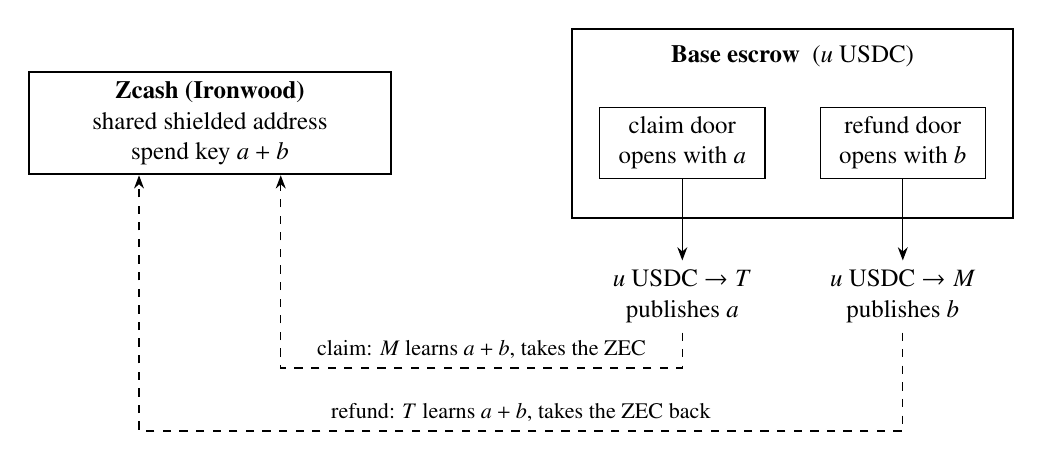
\begin{tikzpicture}[font=\small, box/.style={draw, thick, minimum width=4.6cm, minimum height=1.25cm, align=center},
  door/.style={draw, minimum width=2.1cm, minimum height=0.8cm, align=center}, >=Stealth]
\node[box] (z) at (0,0) {\textbf{Zcash (Ironwood)}\\shared shielded address\\spend key $a+b$};
\node[draw, thick, minimum width=5.6cm, minimum height=2.4cm] (e) at (7.4,0) {};
\node at (7.4,0.85) {\textbf{Base escrow} \ ($u$ USDC)};
\node[door] (c) at (6.0,-0.25) {claim door\\opens with $a$};
\node[door] (r) at (8.8,-0.25) {refund door\\opens with $b$};
\node[align=center] (tt) at (6.0,-2.2) {$u$ USDC $\to T$\\publishes $a$};
\node[align=center] (mm) at (8.8,-2.2) {$u$ USDC $\to M$\\publishes $b$};
\draw[->] (c) -- (tt);
\draw[->] (r) -- (mm);
\draw[->, dashed] (tt.south) -- ++(0,-0.45) -| node[pos=0.25, above, font=\footnotesize]{claim: $M$ learns $a+b$, takes the ZEC} ($(z.south)+(0.9,0)$);
\draw[->, dashed] (mm.south) -- ++(0,-1.25) -| node[pos=0.25, above, font=\footnotesize]{refund: $T$ learns $a+b$, takes the ZEC back} ($(z.south)+(-0.9,0)$);
\end{tikzpicture}
\caption{The ZEC is locked to the sum of two shares. Each exit from the escrow is opened by one share and publishes it, which completes the other party's knowledge of $a+b$.}
\end{figure}

\subsection{Key setup}
\begin{enumerate}\setlength\itemsep{0.15em}
\item $T$ samples $a \leftarrow \mathbb{F}_q^*$ and a seed $s_T$; $M$ samples $b \leftarrow \mathbb{F}_q^*$ and a
seed $s_M$, all fresh for this swap. They exchange $A = [a]\Gor$ and $B = [b]\Gor$ with Schnorr proofs
of knowledge whose challenges bind $\mathsf{sid}$ and the party's role. Each party rejects a proof
that fails, and a proof made for one role does not verify for the other.
\item $T$ commits to $s_T$ before seeing $s_M$ and opens the commitment after; both derive
$\nk = H_{\mathbb{F}_p}(\texttt{"nk"}, \mathsf{sid}, s_T, s_M)$ and
$\rivk = H_{\mathbb{F}_q}(\texttt{"rivk"}, \mathsf{sid}, s_T, s_M)$, where $H$ is BLAKE2b-512 reduced into
the field.
\item If $\ytilde(A + B) = 1$, both replace $(a, A)$ by $(-a, -A)$ and $(b, B)$ by $(-b, -B)$. The rule
is deterministic, so both reach the same result, and $\ak = A + B$ then has $\ytilde = 0$ as the
key encoding requires. In 2{,}000 random trials 990 needed the negation.
\item Both form $\fvk_J = (\ak, \nk, \rivk)$, check that it is a valid full viewing key (in
particular $\ivk \notin \{0, \bot\}$), and derive the shared address $\mathsf{addr}_J$: the
external-scope address at diversifier index~0, encoded as a unified address with only an Orchard
receiver, which receives into Ironwood.
\end{enumerate}
After setup both parties can \emph{see} any note sent to $\mathsf{addr}_J$, and neither can
\emph{spend} it, because spending requires a signature under $\ask_J = a + b$.

The proofs of knowledge are essential. Without them $M$ could choose $B = [b']\Gor - A$, so that
$\ak = [b']\Gor$ is a key he alone controls: the rogue-key attack known from Schnorr
multisignatures~\cite{musig}.

Our derivation of $\nk$ and $\rivk$ is the $\mathsf{use\_qsk} = \mathsf{false}$ branch of
ZIP~2005~\cite{zip2005}, which Ironwood accepts~\cite{zip326}. Notes at a joint address are therefore
not quantum-recoverable. A joint note lives for minutes, so we accept this. A
$\mathsf{use\_qsk} = \mathsf{true}$ variant needs the parties to agree privately on a shared secret
from which $\nk$ and the quantum keys derive, with $\rivk = H^{\rivk}_{\mathsf{qk}}(\ak, \nk)$; no
library implements that derivation yet.

\subsection{Escrow contract}
For each swap the escrow stores the maker, a payout address chosen by $T$, the token and amount
$u$, a relayer fee, $A$ and $B$ as affine Pallas points, $t_0$, $t_1$, and a state in
$\{\textsf{Open}, \textsf{Ready}, \textsf{Claimed}, \textsf{Refunded}\}$:

\begin{itemize}\setlength\itemsep{0.1em}
\item \fn{open}: called by $M$. It checks that $A$ and $B$ lie on the curve and that
$\mathit{now} < t_0 < t_1$, takes $u$ tokens from $M$, and enters \textsf{Open}.
\item \fn{setReady}: called by $M$, in \textsf{Open}, before $t_0$.
\item \fn{claim}$(a)$: callable by anyone before $t_1$, in \textsf{Ready}, or in \textsf{Open} from
$t_0$. It checks $[a]\Gor = A$, pays $u$ minus the relayer fee to the payout address and the fee to
the caller, enters \textsf{Claimed}, and emits $a$.
\item \fn{refund}$(b)$: callable by anyone, in \textsf{Open} before $t_0$, or in \textsf{Open} or
\textsf{Ready} from $t_1$. It checks $[b]\Gor = B$, returns $u$ to $M$, enters \textsf{Refunded},
and emits $b$.
\end{itemize}

\textsf{Claimed} and \textsf{Refunded} are terminal, so at most one exit ever succeeds. Payouts go
to addresses fixed at \fn{open}, so anyone may submit a share without being able to redirect funds,
and a taker whose payout address holds no ETH can have a relayer submit her claim.

No EVM chain has a Pallas precompile, so the contract does the scalar multiplication itself:
Jacobian coordinates, the $a = 0$ doubling and mixed-addition formulas, and a projective comparison
with the stored point ($X = xZ^2$, $Y = yZ^3$), so no field inversion is needed. Checking the
scalar against $A$ directly is what lets us skip the cross-curve proof that the Monero--Ethereum
design requires~\cite{athanor,mrl10}.

\subsection{Settlement}
\begin{enumerate}\setlength\itemsep{0.15em}
\item \textbf{Lock.} $M$ calls \fn{open}. $T$ checks every stored parameter and waits until the call
is on Base's \emph{safe} head, that is, included in a batch posted to Ethereum.
\item \textbf{Fund.} $T$ sends $v + f$ ZEC to $\mathsf{addr}_J$ in a fully shielded transaction from
her own wallet.
\item \textbf{Confirm.} $M$ trial-decrypts with $\ivk_J$, checks the value, waits for $k_Z$
confirmations, and calls \fn{setReady} before $t_0$. If no adequate note arrives, he calls
\fn{refund}.
\item \textbf{Claim.} $T$, or a relayer, submits \fn{claim}$(a)$, and $T$'s payout address
receives the tokens.
\item \textbf{Sweep.} $M$ reads $a$ from the \texttt{Claimed} event, computes $\ask_J = a + b$, and
spends the joint note to an address of his own, signing externally with $\ask_J + \alpha$. The sweep
uses $\ovk = \bot$ and returns no change to $\mathsf{addr}_J$ (Section~7).
\end{enumerate}
If the swap is abandoned, $M$'s \fn{refund}$(b)$ publishes $b$ and $T$ sweeps the note back to
herself with $a + b$.

\subsection{Fees}
The joint note pays for its own sweep. Under ZIP~317~\cite{zip317} the fee is $5{,}000$ zatoshis
per logical action with a minimum of two; for Orchard-protocol bundles the logical-action count is
the number of actions, and the draft Revision~1 for NU6.3 adds the same term for Ironwood. A sweep
with one spend and one output is padded to two actions, so $f = 10{,}000$ zatoshis. On Base, $M$
pays for \fn{open} and \fn{setReady}, and the relayer fee pays whoever submits \fn{claim}.

\section{Deadlines and Liveness}

\begin{figure}[H]
\centering
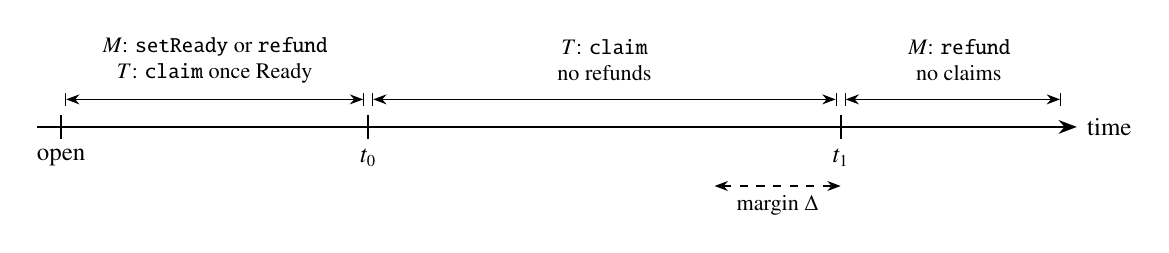
\begin{tikzpicture}[font=\small, >=Stealth]
\draw[thick,->] (0,0) -- (13.2,0) node[right]{time};
\foreach \x/\l in {0.3/open, 4.2/$t_0$, 10.2/$t_1$} { \draw[thick] (\x,0.15) -- (\x,-0.15) node[below]{\l}; }
\node[align=center, font=\footnotesize] at (2.25,0.85) {$M$: \fn{setReady} or \fn{refund}\\$T$: \fn{claim} once Ready};
\node[align=center, font=\footnotesize] at (7.2,0.85) {$T$: \fn{claim}\\no refunds};
\node[align=center, font=\footnotesize] at (11.7,0.85) {$M$: \fn{refund}\\no claims};
\draw[|<->|, thin] (0.35,0.35) -- (4.15,0.35);
\draw[|<->|, thin] (4.25,0.35) -- (10.15,0.35);
\draw[|<->|, thin] (10.25,0.35) -- (13.0,0.35);
\draw[<->, thin, dashed] (8.6,-0.75) -- node[below, font=\footnotesize]{margin $\Delta$} (10.2,-0.75);
\end{tikzpicture}
\caption{Escrow windows. A taker's wallet stops attempting claims at $t_1 - \Delta$.}
\end{figure}

Shielded Zcash cannot enforce a timelock, so all deadlines live in the escrow, and the share that
each exit publishes carries the outcome to Zcash. Table~\ref{tab:liveness} covers every case in
which a party stops responding.

\begin{table}[H]
\centering\small
\begin{tabularx}{\linewidth}{@{}p{3.6cm}X@{}}
\toprule
\textbf{Who stops responding} & \textbf{Outcome}\\
\midrule
$T$, before funding & No note arrives; $M$ refunds before $t_0$. Nothing is at stake.\\
$T$, after funding & $M$ sets Ready. At $t_1$ he refunds and publishes $b$; whenever $T$ returns she sweeps the note with $a+b$. That sweep has no deadline.\\
$M$, after \fn{open} & From $t_0$, $T$ claims without Ready and publishes $a$; the note waits at $\mathsf{addr}_J$ until $M$ returns.\\
Both & After $t_1$ only \fn{refund} remains, and only $M$ knows $b$. A rational $M$ refunds, since otherwise his own tokens stay locked; $T$ then recovers her ZEC.\\
\bottomrule
\end{tabularx}
\caption{Liveness outcomes.}
\label{tab:liveness}
\end{table}

The protocol therefore needs presence at two points. $M$ must act before $t_0$, which a market maker
does automatically. $T$ must claim between Ready and $t_1$; if she does not, she is refunded, unless
$M$ has also disappeared for good, in which case both parties' funds stay locked and $M$ loses as
much as $T$. Monero swaps rely on the same incentive. Five wallet rules make the windows safe:
\begin{itemize}\setlength\itemsep{0.1em}
\item[\textbf{R1}] $T$ funds only after \fn{open} is on Base's safe head and every stored parameter
matches the quote.
\item[\textbf{R1b}] $T$ does not fund within $2\Delta$ of $t_0$, so that $M$ can still confirm the
note and set Ready.
\item[\textbf{R2}] $T$ broadcasts \fn{claim}$(a)$ only if Ready has been observed or $t_0 + \delta$ has
passed, and only before $t_1 - \Delta$.
\item[\textbf{R3}] $M$ broadcasts \fn{refund}$(b)$ only when the refund condition holds with margin
$\delta$.
\item[\textbf{R4}] Shares are fresh for each swap and erased after settlement.
\end{itemize}
R2 and R3 matter because \emph{a reverted transaction still publishes its calldata}. A claim that
lands after $t_1$ fails but reveals $a$, after which $M$ can both refund and sweep; a refund that fails
before $t_1$ reveals $b$, after which $T$ can both claim and sweep. A party must never broadcast a
share unless the contract would accept it, with margin. Rule R1b was added after our first local run
(Section~10.4).

\textbf{Censorship.} Base's sequencer can delay a transaction but cannot exclude it forever.
Transactions deposited through the \fn{OptimismPortal} contract on Ethereum must be included within
the sequencing window, 3{,}600 Ethereum blocks or about 12~hours on Base~\cite{basereliab,opforced};
this still holds after Base's May 2026 Azul upgrade replaced its OP Stack node software. In
production we set $t_1 - t_0 \geq 24$~hours so that a censored taker can force-include her claim. A
relayer that withholds a claim can delay it but not redirect it, and $T$ can resubmit by another
route.

\textbf{Reorganizations.} $M$ waits $k_Z$ Zcash confirmations before Ready, because if the funding
note were reorganized away after Ready, $T$ could claim without having paid. $T$ waits for Base's
safe head before funding, because a reorganized \fn{open} would leave her note at an address with no
escrow; she could recover it only with $M$'s cooperation. For production we suggest
$t_0 = \text{open} + 1$~hour, $t_1 = t_0 + 24$~hours, and $k_Z$ equal to about 15~minutes of blocks.
Our tests used shorter windows (Section~10).

\section{Security}

We assume that discrete logarithms are hard on Pallas, that RedPallas with rerandomized keys is
unforgeable~\cite{spec}, that the proofs of knowledge are extractable, and that a party following
R1--R4 gets its transactions included on Base within the sequencing window.

\textbf{Atomicity.} The escrow lets at most one of \fn{claim} and \fn{refund} succeed. The joint note
can be spent only by someone who knows $a+b$. Before either exit, $T$ knows only $a$ and $M$ only $b$;
the proofs of knowledge and the hardness of discrete logarithms stop either from learning the other's
share or choosing their own as a function of it. A successful \fn{claim} publishes $a$ and pays $T$,
after which only $M$ knows $a+b$. A successful \fn{refund} publishes $b$ and pays $M$, after which only
$T$ knows $a+b$. A third party who sees one published share still lacks the other. The outcome is
therefore both sides settled, both refunded, or, in the last row of Table~\ref{tab:liveness}, both
locked by a party who harms himself as much as his counterparty.

\textbf{Front-running.} \fn{claim} and \fn{refund} pay fixed addresses, so seeing a share early lets
no one redirect funds; seeing $a$ early helps only $M$, who is entitled to it. The one dangerous
ordering is a share broadcast while its door is closed, which R2 and R3 rule out.

\textbf{Secret strength.} Shares are uniform in a 255-bit field. Recovering a share from its public
point is the discrete logarithm problem that protects every Zcash and Bitcoin key; precomputed tables
do not help against uniformly sampled keys.

\textbf{Key compromise.} An attacker who steals $b$ from $M$'s machine during a swap, together with
$\nk$ and $\rivk$, could race $M$ for the note once $a$ is published. Because shares are per swap
(R4), a compromise exposes one swap rather than a wallet, and $M$'s software sweeps within a block of
the claim.

\textbf{Consensus validity.} The construction asks nothing of Zcash consensus beyond what FROST
already uses: a valid full viewing key and a RedPallas signature under the rerandomized joint key.
We confirmed this against the production verifier and a live node (Sections~10.1 and~10.2).

\textbf{Pool lifecycle.} The Orchard pool was sealed in 2026 but stayed spendable. A future upgrade
could seal Ironwood the same way, so implementations should sweep promptly.

\section{Privacy}

\begin{table}[H]
\centering\small
\begin{tabularx}{\linewidth}{@{}p{2.8cm}XX@{}}
\toprule
\textbf{Observer} & \textbf{Learns} & \textbf{Does not learn}\\
\midrule
Zcash chain & Fully shielded transactions, their action counts and fees, and their times. & Any amount, any address, or any link between them or to Base.\\
Base chain & That maker $M$ escrowed $u$ USDC; a fresh payout address; $A$, $B$, and one share. & Anything on Zcash: none of these values appears there.\\
Maker & $v$, the funding transaction, and $T$'s payout and reply addresses. & $T$'s identity, balances or history.\\
Taker & Which transaction sweeps the joint note (she knows $\nk$). & Where the ZEC went: the sweep uses $\ovk = \bot$.\\
Light-wallet server & Client IP, which blocks it downloads, and which full transactions it fetches. & Note contents.\\
Relayer & $a$ shortly before it is published, and the payout address. & Anything on Zcash.\\
\bottomrule
\end{tabularx}
\caption{What each observer learns.}
\end{table}

\textbf{The Base values do not appear on Zcash.} After settlement $A$, $B$, $\ak = A + B$ and one share
are public on Base. On Zcash a spend publishes $\rk = \ak + [\alpha]\Gor$ for uniform $\alpha$, a
uniform point independent of $\ak$, and an address depends on $\ivk$, hence on $\nk$ and $\rivk$, which
are never published. An observer who knows $\ak$ can recognize neither the joint address nor its
spend; in our tests no on-chain $\rk$ ever equalled $\ak$.

\textbf{The shared outgoing viewing key.} Anyone holding $\fvk_J$ can derive $\ovk_J$. If the sweep
encrypted its output's recovery data under $\ovk_J$, the counterparty could read the destination and
amount. Our tests recover the destination in exactly that case and fail to when the sweep uses
$\ovk = \bot$, which is what our implementation does.

\textbf{The light-wallet server.} Compact blocks carry no memos, so our wallet fetches the full
transaction for each note it decrypts, and the server learns which transactions concern us. A
deployment should route light-wallet traffic over Tor, fetch decoy transactions, or download full
blocks; our implementation does none of these yet.

\textbf{Timing and amounts.} An observer can correlate the time of \fn{open} or \fn{claim} with
shielded transactions in the same interval; the anonymity set is every shielded transaction in that
window. Either party can delay its Zcash transaction at no risk: $T$ can fund at any time before
$t_0$, and $M$ can sweep at any time after the claim. ZEC amounts never appear on chain. The USDC
amount is public by design, and standard lot sizes keep it from fingerprinting a trade.

\textbf{Comparison.} NEAR Intents, Maya and THORChain move ZEC through a transparent address and a
custodian, so the deposit amount and time are public and the custodian can hold the output.
Hash-locked swaps link both legs by the hash and use transparent ZEC. In Cloakroom the ZEC stays
shielded throughout, no third party holds either asset, and timing is the only link between the
chains.

\section{The Dark Pool}

Settlement removes the custodian; the request-for-quote layer removes the venue. A maker publishes a
unified address, an EVM address and the pairs it quotes. Messages travel as memos on shielded outputs
that may carry zero ZEC; a memo whose first byte is \texttt{0xFF} carries application
data~\cite{zip302}. Every message begins with \texttt{0xFF}, \texttt{"CLKR"}, a version and a type.

\begin{table}[H]
\centering\small
\begin{tabularx}{\linewidth}{@{}lX r@{}}
\toprule
\textbf{Message} & \textbf{Fields after the 7-byte header} & \textbf{Bytes}\\
\midrule
\textsf{RFQ} ($T\to M$) & rfq id (16), lots (1), $A$ (32), $\pi_A$ (64), commitment to $s_T$ (32), payout address (20), reply address (43) & 215\\
\textsf{Quote} ($M\to T$) & rfq id (16), price (8), relayer fee (8), $B$ (32), $\pi_B$ (64), $s_M$ (32), escrow (20), maker EVM address (20), $t_0$ and $t_1$ offsets (8) & 215\\
\textsf{Accept} ($T\to M$) & rfq id (16), $s_T$ (32), hash of the quote (32) & 87\\
\textsf{Fund} ($T\to\mathsf{addr}_J$) & rfq id (16) & 23\\
\bottomrule
\end{tabularx}
\caption{RFQ messages, as implemented. Each fits in one 512-byte memo.}
\end{table}

A taker sends an \textsf{RFQ} to a maker with a fresh diversified reply address. The maker
replies with a \textsf{Quote} to that address, and the taker answers with \textsf{Accept}, after
which the maker calls \fn{open} and settlement proceeds as in Section~4.4. A quote carries no
signature: only the maker received the RFQ, so only the maker knows the reply address, and before
funding the taker checks that the escrow was opened by the maker's EVM address with exactly the quoted
parameters. A taker who asks several makers uses a different reply address for each. Lots have fixed
sizes, so the price is the only trade-specific number on Base.

A maker learns what is asked (pair, side, size) and the taker's fresh addresses, which any quoting
requires, but not who is asking. The chain sees only shielded transactions. A taker can send
requests every period whether or not she trades, to hide when she is active, and requests can carry a
small fee to deter spam.

\section{Implementation}

The implementation, written for this paper, has four parts:
\begin{itemize}\setlength\itemsep{0.1em}
\item \textbf{Rust node} (\fn{cloakroom}): key setup, proofs of knowledge, the message codec, maker
and taker state machines, and a light wallet that builds v6 transactions through the PCZT roles. It
signs joint spends externally with \fn{apply\_ironwood\_signature}. It syncs either from a Zebra
node over JSON-RPC or from a lightwalletd server over gRPC, starting from the server's Ironwood tree
state at a birthday height. Built on \fn{orchard}~0.16.0, \fn{pczt}~0.10.0-pre.1 and
\fn{zcash\_primitives}~0.31.0-pre.1.
\item \textbf{Solidity}: the escrow and a Pallas library, 3{,}938 bytes of runtime code
(Solidity 0.8.30, via-IR). The EVM side is driven through Foundry's \fn{cast}.
\item \textbf{Harness}: a script that starts a Zebra regtest node and a local EVM chain, deploys the
contracts, funds two independent wallets, and runs each scenario with maker and taker as separate
operating-system processes that share no state.
\item \textbf{Tools}: \fn{lwdscan} reports balances from compact blocks, and \fn{txaudit} reports
what a transaction reveals.
\end{itemize}
Both processes persist their state after every step. A party can be stopped at any stage and
restarted, which is how the tests make parties ``disappear''.

\section{Evaluation}

\subsection{Against the production verifier}
A test program against \fn{orchard}~0.16.0 with the post-NU6.3 circuit and Ironwood bundles checks:
\begin{enumerate}\setlength\itemsep{0.05em}
\item The proofs of knowledge verify, a proof for one role fails for the other, and a rogue share
$B = [b']\Gor - A$ fails.
\item \fn{FullViewingKey::from\_bytes} accepts $(A+B, \nk, \rivk)$, and $\ivk_J$ decrypts a funding
note and its memo.
\item A sweep signed with $b$ alone is rejected; one signed with $(a+b)+\alpha$ passes proof,
spend-authorization and binding-signature verification, and so does the refund sweep.
\item With $\ovk_J$ the counterparty recovers the sweep's destination; with $\ovk = \bot$ it does
not. No published $\rk$ equals $\ak$.
\end{enumerate}
On a 10-core laptop the circuit keys took 1.8~s to build and a two-action proof took 0.61~s.

\subsection{On a Zebra node}
On Zebra 7.0.0-rc.0 in regtest with NU6.3 rules, a block reward was mined to a joint address. A v6
transaction built through the PCZT roles, with the real ZIP~244 sighash and an external signature
under $(a+b)+\alpha$, was accepted to the mempool and mined (txid \hx{6c7d4df5\ldots a01616},
block~4). A copy differing only in its 64-byte spend-authorization signature, made with $b$ alone, was
rejected (error $-25$). Zebra reports this as a proof failure because it verifies proofs and
signatures in one batch; checked separately, the proof and binding signature of the copy were valid
and only its spend signature failed.

\subsection{Contract tests and gas}
Fifteen Foundry tests cover the happy path, each row of Table~\ref{tab:liveness}, wrong shares at each
door, window boundaries and off-curve points. A fuzz test of 5{,}000 random times, Ready states and
call orders never paid both sides and always conserved the token supply. The Pallas library
reproduces the Rust vectors for $\Gor$, $A$, $B$ and $[q-1]\Gor = -\Gor$.

\begin{table}[H]
\centering\small
\begin{tabular}{@{}lrr@{}}
\toprule
\textbf{Operation} & \textbf{Foundry, mock token} & \textbf{Base Sepolia, Circle USDC}\\
\midrule
Pallas check $[k]\Gor \stackrel{?}{=} (x,y)$ & 467{,}341 & ---\\
\fn{open} & 279{,}042 & 297{,}756\\
\fn{setReady} & 32{,}440 & 32{,}440\\
\fn{claim} & 553{,}364 & 564{,}054\\
\fn{refund} & 528{,}531 & 505{,}221\\
\bottomrule
\end{tabular}
\caption{Gas used.}
\end{table}

A swap costs about $9\times10^5$ gas, a few cents on Base. An earlier Solidity Pasta library reports
389{,}487 gas for a projective scalar multiplication~\cite{pastasol}. A table of precomputed
multiples of $\Gor$ would cut our cost further; we have not needed it.

\subsection{Two-party scenarios}
Table~\ref{tab:scen} lists the seven scenarios, all run in one session on fresh chains, with 43 checks
including balances exact to the zatoshi. Scenarios s2, s3, s4 and s6 needed the share negation of
Section~4.2 and s1 and s7 did not, so both branches ran on chain.

\begin{table}[H]
\centering\small
\begin{tabularx}{\linewidth}{@{}lXl@{}}
\toprule
& \textbf{Scenario} & \textbf{Outcome}\\
\midrule
s1 & Happy path: RFQ, quote, accept, open, fund, ready, claim, sweep & settled\\
s2 & Taker accepts, then disappears before funding & refunded before $t_0$\\
s3 & Taker funds and disappears; returns after $t_1 - \Delta$ & R2 refuses the claim; refunded; ZEC recovered\\
s4 & Maker opens, then disappears without setting Ready & claimed after $t_0$; maker sweeps on return\\
s5 & Maker sends a rogue key $B = [b']\Gor - A$ & quote rejected; nothing funded\\
s6 & Taker underfunds the joint address & no Ready; refunded; ZEC recovered\\
s7 & Happy path with NU7 active & settled\\
\bottomrule
\end{tabularx}
\caption{Scenarios on Zebra regtest and a local EVM chain. All passed.}
\label{tab:scen}
\end{table}

In every scenario that moves ZEC, the taker lost exactly the expected fees. In s1, s3 and s7 we read
every Zcash transaction either party made back from the node: all were v6 with two Ironwood actions,
no transparent inputs or outputs, and an Ironwood value balance equal to the 10{,}000-zatoshi fee.

The first runs also found a liveness gap. With $t_0$ only 40~seconds after \fn{open}, the taker
waited for the safe head (which lags about 32~blocks on the local chain) and funded just as the
maker's no-funding refund fired. The protocol resolved it safely: the maker refunded, and the taker
read $b$ and recovered her note. We added rule R1b so that a taker never funds that close to $t_0$.

\subsection{Public networks}
We ran two swaps between Zcash testnet, which runs NU7 rules, and Base Sepolia. The Zcash wallets
synced through the public \fn{testnet.zec.rocks} lightwalletd server; the escrow is deployed at
\hx{0x2df30788\ldots39a1} with its source verified on Blockscout. Lots were 0.01~TAZ for 1~USDC,
with a 0.1~USDC relayer fee, $t_0 = \text{open} + 15$~minutes, $t_1 = t_0 + 15$~minutes, and
$k_Z = 3$.

\begin{table}[H]
\centering\small
\begin{tabularx}{\linewidth}{@{}lX@{}}
\toprule
\textbf{Swap} & \textbf{Result, checked on chain}\\
\midrule
1, happy path & RFQ, quote and accept memos in blocks 4{,}501{,}217--225; funding in 4{,}501{,}234; \fn{setReady} after 4 confirmations; claim by the relayer; maker's joint-key sweep in 4{,}501{,}240. The fresh payout address received 0.9~USDC, the relayer 0.1~USDC, and the maker 0.01~TAZ.\\
2, refund & The taker funded in block 4{,}501{,}274 and its process exited. The maker set Ready, waited past $t_1$, and refunded, publishing $b$. The returning taker swept the note back with $a+b$ in block 4{,}501{,}358, losing exactly four 0.0001~TAZ fees.\\
\bottomrule
\end{tabularx}
\caption{Swaps between Zcash testnet and Base Sepolia, October 14, 2026.}
\end{table}

All eleven Zcash transactions involved (a transfer to fund the maker and five per swap) are v6, with
two Ironwood actions, no transparent inputs or outputs, no Sapling or Orchard-pool activity, and an
Ironwood value balance equal to the fee.

The public networks exposed four problems that local chains did not, all now fixed:
\begin{itemize}\setlength\itemsep{0.1em}
\item The public RPC served a stale nonce, so the maker's \fn{open} collided with its \fn{approve}.
Sends now retry, and \fn{open} checks the escrow first, so a retry is idempotent.
\item The public RPC limits log queries to 200 blocks, so lookups now query in chunks.
\item A network error stopped a process. Errors are now logged and retried; the maker rode out two
RPC timeouts in swap~2.
\item A balance read just after a claim returned stale data. Balances are now checked separately.
\end{itemize}
After these fixes, all seven local scenarios still pass.

\section{Limitations}

\textbf{Liveness.} Takers must claim within a window and makers must respond before $t_0$.
\textbf{Liquidity.} Atomic swaps have historically traded small volumes; the RFQ layer lets
professional makers provide depth but does not create them. \textbf{Our implementation} supports one
maker per request, trusts the relayer for liveness only, does not use Tor, and lets the light-wallet
server see which transactions it fetches. Its contracts are unaudited. \textbf{Not tested:} forced
inclusion through Ethereum, Base mainnet, Zcash mainnet, and the production window lengths of
Section~5. \textbf{Quantum recovery} is unavailable for joint notes (Section~4.2).
\textbf{Linkability by timing} remains (Section~7). \textbf{Chains without elliptic-curve
arithmetic}, such as Bitcoin, would need adaptor signatures and a cross-group proof~\cite{gugger,mrl10}
in place of our escrow.

\section{Conclusion}

We have proposed a way to trade shielded Zcash without leaving the shielded pool and without a
custodian. The spending key of a fresh Ironwood address is split between the two parties, and the
counterparty's tokens are held by a contract whose two exits each publish one share. Because taking
either exit completes the other party's knowledge of the key, the swap settles atomically or unwinds
atomically. The Zcash leg is ordinary shielded transactions, the EVM leg reveals the price, and the
request-for-quote messages ride inside encrypted memos. The construction needs no change to Zcash
consensus, and it already runs between Zcash testnet and Base Sepolia.

\renewcommand{\refname}{References}
\begin{thebibliography}{99}\small\setlength\itemsep{0.05em}
\bibitem{zerocash} E. Ben-Sasson, A. Chiesa, C. Garman, M. Green, I. Miers, E. Tromer, M. Virza, ``Zerocash: Decentralized anonymous payments from Bitcoin,'' \emph{IEEE S\&P}, 2014.
\bibitem{spec} D. Hopwood, S. Bowe, T. Hornby, N. Wilcox, ``Zcash Protocol Specification,'' version 2026.7.0, \url{https://zips.z.cash/protocol/protocol.pdf}.
\bibitem{bitcoin} S. Nakamoto, ``Bitcoin: A peer-to-peer electronic cash system,'' 2008.
\bibitem{zip258} D. Hopwood, ``ZIP 258: Deployment of the NU6.3 network upgrade,'' \url{https://zips.z.cash/zip-0258}.
\bibitem{zip326} D. Hopwood, ``ZIP 326: NU6.3 consequences for wallets,'' \url{https://zips.z.cash/zip-0326}.
\bibitem{zip2005} D. Hopwood, J. Grigg, ``ZIP 2005: Ironwood quantum recoverability,'' \url{https://zips.z.cash/zip-2005}.
\bibitem{zip259} D. Ojha, ``ZIP 259: Deployment of the NU7 network upgrade,'' \url{https://zips.z.cash/zip-0259}.
\bibitem{kappos} G. Kappos, H. Yousaf, M. Maller, S. Meiklejohn, ``An empirical analysis of anonymity in Zcash,'' \emph{USENIX Security}, 2018.
\bibitem{quesnelle} J. Quesnelle, ``On the linkability of Zcash transactions,'' arXiv:1712.01210, 2017.
\bibitem{biryukov} A. Biryukov, D. Feher, ``Privacy and linkability of mining in Zcash,'' \emph{IEEE CNS}, 2019.
\bibitem{railgun} K. Huseynov, A. Shahzaib, I. A. Seres, J. Tapolcai, ``A tattered cloak of invisibility: Measuring anonymity loss in Railgun on Ethereum,'' arXiv:2606.25926, 2026.
\bibitem{nearchains} NEAR Intents, ``Supported chains,'' \url{https://docs.near-intents.org/resources/chain-support}.
\bibitem{freeze} C. Monasterio, ``\$589K USDT stuck for 50 days after Zodl swap,'' Crypto Economy, Sep.\ 11, 2026.
\bibitem{nearexploit} CoinCentral, ``NEAR Intents hacked for \$3.8 million,'' Oct.\ 2, 2026.
\bibitem{nolan} T. Nolan, ``Alt chains and atomic transfers,'' bitcointalk.org, 2013.
\bibitem{herlihy} M. Herlihy, ``Atomic cross-chain swaps,'' \emph{PODC}, 2018.
\bibitem{xcat} J. Graber, ``ZIP 300: Cross-chain atomic transactions,'' \url{https://zips.z.cash/zip-0300}, 2017.
\bibitem{gugger} J. Gugger, ``Bitcoin--Monero cross-chain atomic swap,'' IACR ePrint 2020/1126.
\bibitem{comit} COMIT, ``xmr-btc-swap,'' \url{https://github.com/comit-network/xmr-btc-swap}; continued as eigenwallet.
\bibitem{athanor} E. Binks, ``Cross-chain atomic swaps between Ethereum and Monero,'' AthanorLabs, 2022.
\bibitem{mrl10} S. Noether, ``Discrete logarithm equality across groups,'' MRL-0010, 2018.
\bibitem{uas} S. A. K. Thyagarajan, G. Malavolta, P. Moreno-Sanchez, ``Universal atomic swaps: Secure exchange of coins across all blockchains,'' \emph{IEEE S\&P}, 2022.
\bibitem{zswappets} F. Engelmann, T. Kerber, M. Kohlweiss, M. Volkhov, ``Zswap: zk-SNARK based non-interactive multi-asset swaps,'' \emph{PoPETs} 2022(4).
\bibitem{zwap} Atheon, ``Zwap: Trustless shielded atomic swaps for Zcash (early access),'' Zcash Community Forum, May 2026.
\bibitem{zswap} Stallion Labs, ``Grant application: zswap,'' Zcash Community Grants issue \#443, 2026.
\bibitem{renegade} Renegade, documentation, \url{https://docs.renegade.fi}.
\bibitem{penumbra} Penumbra, ``Decentralized exchange,'' \url{https://protocol.penumbra.zone/main/dex.html}.
\bibitem{zip244} K. Nuttycombe, D. Hopwood, J. Grigg, ``ZIP 244: Transaction identifier non-malleability,'' \url{https://zips.z.cash/zip-0244}.
\bibitem{halo} S. Bowe, J. Grigg, D. Hopwood, ``Recursive proof composition without a trusted setup,'' IACR ePrint 2019/1021.
\bibitem{zip374} J. Grigg, ``ZIP 374: Partially created Zcash transaction format,'' \url{https://zips.z.cash/zip-0374}.
\bibitem{frost} C. Komlo, I. Goldberg, ``FROST: Flexible round-optimized Schnorr threshold signatures,'' \emph{SAC}, 2020.
\bibitem{zip312} C. Gouv\^{e}a, C. Komlo, D. Connolly, ``ZIP 312: FROST for spend authorization multisignatures,'' \url{https://zips.z.cash/zip-0312}.
\bibitem{musig} G. Maxwell, A. Poelstra, Y. Seurin, P. Wuille, ``Simple Schnorr multi-signatures with applications to Bitcoin,'' \emph{Designs, Codes and Cryptography}, 2019.
\bibitem{zip317} D. Hopwood, K. Nuttycombe, J. Grigg, ``ZIP 317: Proportional transfer fee mechanism,'' \url{https://zips.z.cash/zip-0317}.
\bibitem{basereliab} Base, ``Reliability and liveness,'' \url{https://docs.base.org/specifications/security/reliability-and-liveness}.
\bibitem{opforced} Optimism, ``Forced transaction,'' \url{https://docs.optimism.io/stack/transactions/forced-transaction}.
\bibitem{zip302} J. Graber, J. Grigg, ``ZIP 302: Standardized memo field format,'' \url{https://zips.z.cash/zip-0302}.
\bibitem{pastasol} Z. Zhang, ``pasta-solidity,'' \url{https://github.com/zhenfeizhang/pasta-solidity}.
\end{thebibliography}

\appendix
\section*{Appendix: Test Vectors}
{\small
$\Gor$, as used in the escrow and extracted from \fn{orchard}~0.16.0 (its compressed encoding matches the \fn{reddsa} crate's basepoint constant):\\
\texttt{x = 0x375523b328f1d6063b8d187c3e5f445f0c7f0ce37b70a10c8d1a7284b875c963}\\
\texttt{y = 0x1ad0357fdf1a66db7b10bcfcfed624fbdfc914fec005bdd84ce33e817b0c3bc9}

A share and its point after sign normalization:\\
\texttt{a\ \ \ = 0x195661e2e4789b7f57137b2e777736d79720270638d12e4882fd95e52a73d6b3}\\
\texttt{A.x = 0x17a182b1eb9594581ecaad0fcb61546f4c366cc57b9575ddde22ca56963c304c}\\
\texttt{A.y = 0x19b252972f768cc5708b251baca77a9afd02dddd9531510aafb13c4824d7b61f}
}

\end{document}
